\documentclass[crop=true, tikz=true, border={0.1cm 1cm 1cm 0.1cm}]{standalone}

\usepackage{times}
\usepackage{helvet}
\usepackage{courier}
\usepackage{url}  %Required
\usepackage{graphicx}  %Required

%%%%%%%%%%%%%%%%%%%%%
%%%% Packages
\usepackage{amsthm,amsmath,amssymb}
%\usepackage{tikz}
\usetikzlibrary{matrix}
\usepackage{pgf-umlsd}
\usepackage{pgfplots}
\usepackage{pgfplotstable}
\usepgfplotslibrary{fillbetween}
\usepackage{ragged2e}
\usetikzlibrary{arrows,automata,fit,calc,positioning,shapes,shapes.multipart} %
%\usepackage[inline]{enumitem}
\usepackage{enumerate,url,soul}
\usepackage{paralist}
%\usepackage[usenames]{color} % Only used in comment commands
\usepackage[ruled,vlined]{algorithm2e}
\usepackage{thmtools,thm-restate}
\usepackage{listings}
\usepackage{subcaption}
\usepackage{arydshln}

\def\longflagdefined{}
%%%%%%%%%%%%%%%%%%%%%%%%%%%%%%%%%%%%%%%%%%%%%%%%%%%%%%%%%%%%%%%%%%%%%%%%%%%%%%%%%
%%%%%%%%%%%%%%%%%%%%%%%%%%%%%%%%%%%%%%%%%%%%%%%%%%%%%%%%%%%%%%%%%%%%%%%%%%%%%%%%%
%%%%%%%%%%%%%%%%%%%%%%%%%%%%%%%%%%%%%%%%%%%%%%%%%%%%%%%%%%%%%%%%%%%%%%%%%%%%%%%%%
%%% slides stuff

\newcommand{\blocknode}[5]{\node (#1) at #2 {%
    \begin{minipage}{3.5cm}\begin{block}{#4}
        \begin{overlayarea}{3.5cm}{#3}
        #5\end{overlayarea}\end{block}\end{minipage}};}
\newcommand{\smallblocknode}[5]{\node (#1) at #2 {%
    \begin{minipage}{3.0cm}\begin{block}{#4} \begin{overlayarea}{3.0cm}{#3}
    #5\end{overlayarea}\end{block}\end{minipage}};}
\newcommand{\redsmallblocknode}[5]{\node (#1) at #2 {%
    \begin{minipage}{3.0cm}\begin{alertblock}{#4} \begin{overlayarea}{3.0cm}{#3}
    #5\end{overlayarea}\end{alertblock}\end{minipage}};}



\renewcommand{\newblock}{}
\definecolor{ToDoColor}{rgb}{0,0.16,0.90} %blue
\definecolor{OutlineColor}{rgb}{0.2,0.8,0.2} %green
\definecolor{CommentColor}{rgb}{0.90,0.16,0} %red
\definecolor{dkgreen}{rgb}{0,0.5,0}
\definecolor{mLightBrown}{rgb}{0.71,0.40,0.11}
\definecolor{mLightGreen}{rgb}{0.56,0.93,0.56}
\newcommand<>{\textblue}[1]{{\color#2{blue}#1}}
\newcommand<>{\textred}[1]{{\color#2{red}#1}}
\newcommand<>{\textgreen}[1]{{\color#2{green}#1}}
\newcommand<>{\textdkgreen}[1]{{\color#2{dkgreen}#1}}
\newcommand<>{\textorange}[1]{{\color#2{orange}#1}}
\newcommand<>{\textyellow}[1]{{\color#2{yellow}#1}}

\newcommand{\ie}{i.\,e.}
\newcommand{\eg}{e.\,g.}
\newcommand{\cf}{cf.}

\newcommand{\notesym}{\ensuremath{\to}} 
\newcommand{\noteblk}[1]{
\begin{block}{}
#1
\end{block}} 

\newcommand{\lectureslides}[1]{\ifthenelse{\value{VERSION}=0}{#1}{}}
\newcommand{\nolectureslides}[1]{\ifthenelse{\not\value{VERSION}=0}{#1}{}}
\newcommand{\posthandout}[1]{\ifthenelse{\value{VERSION}=1}{#1}{}}
\newcommand{\noposthandout}[1]{\ifthenelse{\not\value{VERSION}=1}{#1}{}}
\newcommand{\prehandout}[1]{\ifthenelse{\value{VERSION}=2}{#1}{}}
\newcommand{\noprehandout}[1]{\ifthenelse{\not\value{VERSION}=2}{#1}{}}


\newcommand{\images}{../IMAGES}
\graphicspath{{../IMAGES/}}
\newcommand{\rovergoal}[1]{
\includegraphics[scale=0.06]{rovergoal#1.png}
}


%%%%%%%%%%%%%%%%%%%%%%%%%%%%%%%%%%%%%%%%%%%
%%% defs, propositions, etc

\newenvironment{mydef}[1]{

\begin{block}{#1}
}{
\end{block}
}

\newenvironment{myprop}[1]{

\begin{block}{Proposition (#1)}
}{
\end{block}
}

\newenvironment{myproof}{

\begin{block}{Proof}
}{
\end{block}
}



%%%%%%%%%%%%%%%%%%%%%
%%%
%%% quiz: highlight ``correct'' (green, 2), ``discuss''
%%% (orange, 1), ``false'' (red, 0) in post-handouts only!

\newcommand{\quiz}[9]{

\prehandout{
\begin{block}{Quiz}
\textbf{#1}
\vspace{-0.15cm}
\begin{columns}
\begin{column}{.45\textwidth}
\begin{itemize}
\item[\textblue{(A):}] #2\vspace{-0.05cm}
\item[\textblue{(C):}] #4
\end{itemize}
\end{column}
\begin{column}{.45\textwidth}
\begin{itemize}
\item[\textblue{(B):}] #3\vspace{-0.05cm}
\item[\textblue{(D):}] #5
\end{itemize}
\end{column}
\end{columns}
\end{block}
}

\lectureslides{
\begin{block}{Quiz}
\textbf{#1}
\vspace{-0.15cm}
\begin{columns}
\begin{column}{.45\textwidth}
\begin{itemize}
\item[\textblue{(A):}] #2\vspace{-0.05cm}
\item[\textblue{(C):}] #4
\end{itemize}
\end{column}
\begin{column}{.45\textwidth}
\begin{itemize}
\item[\textblue{(B):}] #3\vspace{-0.05cm}
\item[\textblue{(D):}] #5
\end{itemize}
\end{column}
\end{columns}
\end{block}
}

\posthandout{
\begin{block}{Quiz}
\textbf{#1}
\vspace{-0.15cm}
\begin{columns}
\begin{column}{.45\textwidth}
\begin{itemize}
\item[\textblue{(A):}] \ifthenelse{#6=0}{\textred{#2}}{\ifthenelse{#6=1}{\textorange{#2}}{\ifthenelse{#6=2}{\textdkgreen{#2}}{}}}\vspace{-0.05cm}
\item[\textblue{(C):}] \ifthenelse{#8=0}{\textred{#4}}{\ifthenelse{#8=1}{\textorange{#4}}{\ifthenelse{#8=2}{\textdkgreen{#4}}{}}}
\end{itemize}
\end{column}
\begin{column}{.45\textwidth}
\begin{itemize}
\item[\textblue{(B):}] \ifthenelse{#7=0}{\textred{#3}}{\ifthenelse{#7=1}{\textorange{#3}}{\ifthenelse{#7=2}{\textdkgreen{#3}}{}}}\vspace{-0.05cm}
\item[\textblue{(D):}] \ifthenelse{#9=0}{\textred{#5}}{\ifthenelse{#9=1}{\textorange{#5}}{\ifthenelse{#9=2}{\textdkgreen{#5}}{}}}
\end{itemize}
\end{column}
\end{columns}
\end{block}
}

}




%%%%%%%%%%%%%%%%%%%%%
%%%
%%% quiztwo: highlight ``correct'' (green, 2), ``discuss''
%%% (orange, 1), ``false'' (red, 0) in post-handouts only!

\newcommand{\quiztwo}[5]{

\prehandout{
\begin{block}{Quiz}
\textbf{#1}
\vspace{-0.15cm}
\begin{columns}
\begin{column}{.45\textwidth}
\begin{itemize}
\item[\textblue{(A):}] #2
\end{itemize}
\end{column}
\begin{column}{.45\textwidth}
\begin{itemize}
\item[\textblue{(B):}] #3
\end{itemize}
\end{column}
\end{columns}
\end{block}
}

\lectureslides{
\begin{block}{Quiz}
\textbf{#1}
\vspace{-0.15cm}
\begin{columns}
\begin{column}{.45\textwidth}
\begin{itemize}
\item[\textblue{(A):}] #2
\end{itemize}
\end{column}
\begin{column}{.45\textwidth}
\begin{itemize}
\item[\textblue{(B):}] #3
\end{itemize}
\end{column}
\end{columns}
\end{block}
}

\posthandout{
\begin{block}{Quiz}
\textbf{#1}
\vspace{-0.15cm}
\begin{columns}
\begin{column}{.45\textwidth}
\begin{itemize}
\item[\textblue{(A):}] \ifthenelse{#4=0}{\textred{#2}}{\ifthenelse{#4=1}{\textorange{#2}}{\ifthenelse{#4=2}{\textdkgreen{#2}}{}}}
\end{itemize}
\end{column}
\begin{column}{.45\textwidth}
\begin{itemize}
\item[\textblue{(B):}] \ifthenelse{#5=0}{\textred{#3}}{\ifthenelse{#5=1}{\textorange{#3}}{\ifthenelse{#5=2}{\textdkgreen{#3}}{}}}
\end{itemize}
\end{column}
\end{columns}
\end{block}
}

}




%%%%%%%%%%%%%%%%%%%%%%%%%%%%%%%%%%%%%%%%%%%%%%%%%%%%%%%%%%%%%%%%%%%%%%%%%%%%%%%%%
%%%%%%%%%%%%%%%%%%%%%%%%%%%%%%%%%%%%%%%%%%%%%%%%%%%%%%%%%%%%%%%%%%%%%%%%%%%%%%%%%
%%%%%%%%%%%%%%%%%%%%%%%%%%%%%%%%%%%%%%%%%%%%%%%%%%%%%%%%%%%%%%%%%%%%%%%%%%%%%%%%%
%%% commands from paper

\newcommand{\defined}[1]{\textblue{#1}}


%%%%%%%%%%% heuristics %%%%%%%%%%%%

\newcommand{\hrefine}{\ensuremath{h_{r}}}
\newcommand{\hboth}{\ensuremath{h_{r+b}}}
\newcommand{\hbellman}{\ensuremath{h_{b}}}

\newcommand{\abs}{\mathcal{A}}
\newcommand{\numtasks}[1]{\tiny{(#1)}}

%\newcommand{\formalspacesave}{}

\newcommand{\naturals}{\ensuremath{\mathbb N}}
\newcommand{\reals}{{\mathbb{R}}}
\newcommand{\powerset}{{\mathcal{P}}}

\newcommand{\tuple}[1]{\ensuremath{\langle #1 \rangle}}

\newcommand{\astar}{\ensuremath{\textrm{A}^*}}

\newcommand{\poly}{\textbf{P}}
\newcommand{\np}{\textbf{NP}}
\newcommand{\pspace}{\textbf{PSPACE}}


%%%%%%%%%%%%%%%%%%%%%%%%%%%%%%
%%%%% Generic Framework
\newcommand{\task}{\ensuremath{\tau}}
%\newcommand{\task}{\ensuremath{\cal T}}
\newcommand{\plan}{\ensuremath{\pi}}
\newcommand{\plans}{\ensuremath{\Pi}}
%\newcommand{\alltasks}{\ensuremath{\cal T}}
\newcommand{\allplans}{\ensuremath{\cal P}}
\newcommand{\true}{\ensuremath{\mathit{true}}}
\newcommand{\false}{\ensuremath{\mathit{false}}}

\newcommand{\prop}{\ensuremath{p}}
\newcommand{\propq}{\ensuremath{q}}
\newcommand{\props}{\ensuremath{P}}
\newcommand{\propsatom}{\ensuremath{{P^{\text{\textup{A}}}}}}
\newcommand{\propscomp}{\ensuremath{{P^{\text{\textup{C}}}}}}

\newcommand{\modelsof}[2]{\ensuremath{{\cal M}_#1(#2)}}
\newcommand{\entails}[3]{\ensuremath{#1 \models #2 \Rightarrow #3}}
\newcommand{\notentails}[3]{\ensuremath{#1 \not\models #2 \Rightarrow #3}}
\renewcommand{\iff}[3]{\ensuremath{#1 \models #2 \Leftrightarrow #3}}
\renewcommand{\equiv}[2]{\ensuremath{[#2]_{#1}}}
%
%% \renewcommand{\implies}[1]{\ensuremath{\Rightarrow_{#1}}}
%% \renewcommand{\iff}[1]{\ensuremath{\Leftrightarrow_{#1}}}
%% \renewcommand{\equiv}[2]{\ensuremath{[#1]_{#2}}}

\newcommand{\pdo}[1]{\ensuremath{\Rightarrow_{#1}}}
\newcommand{\pda}[1]{\ensuremath{\Phi_{#1}}}

\newcommand{\entailsuff}{\ensuremath{\Rightarrow_{\mathit{suff}}}}

\newcommand{\deps}{\ensuremath{D}}


%%%%%%%%%%%%%%%%%%%%%%%%%%%%%%
%%%%% Planning Tasks

\newcommand{\vars}{\ensuremath{V}}
\newcommand{\acts}{\ensuremath{A}}
\newcommand{\init}{\ensuremath{I}}
\newcommand{\goal}{\ensuremath{G}}
\newcommand{\goalhard}{\ensuremath{G^{\text{\textup{hard}}}}}
\newcommand{\goalsoft}{\ensuremath{G^{\text{\textup{soft}}}}}
\newcommand{\cost}{{\ensuremath{c}}}
\newcommand{\pre}{\ensuremath{\mathit{pre}}}
\newcommand{\eff}{\ensuremath{\mathit{eff}}}

\newcommand{\variables}[1]{\ensuremath{{\cal V}(#1)}}
\newcommand{\apply}[1]{\ensuremath{[[#1]]}}

\newcommand{\costbound}{{\ensuremath{b}}}


%%%%%%%%%%%%%%%%%%%%%%%%%%%%%%
%%%%% Goal facts

\newcommand{\goalpropsatom}{\ensuremath{{P^{\text{\textup{GA}}}}}}
\newcommand{\goalpropscomp}{\ensuremath{{P^{\text{\textup{GC}}}}}}

\newcommand{\geprops}{\ensuremath{{P^{\text{\textup{GE}}}}}}
\newcommand{\gedeps}{\ensuremath{{D^{\text{\textup{GE}}}}}}

\newcommand{\dgeprops}{\ensuremath{{P^{\text{\textup{DGE}}}}}}
\newcommand{\dgedeps}{\ensuremath{{D^{\text{\textup{DGE}}}}}}



%%%%%%%%%%%%%%%%%%%%%%%%%%%%%%
%%%%% Heuristic Functions

\newcommand{\hstar}{\ensuremath{h^*}}
\newcommand{\hplus}{\ensuremath{h^+}}

\newcommand{\hone}{\ensuremath{h^1}}
\newcommand{\htwo}{\ensuremath{h^2}}
\newcommand{\hm}{\ensuremath{h^m}}
\newcommand{\hc}{\ensuremath{h^C}}
\newcommand{\hcx}{\ensuremath{h^{C \cup X}}}
\newcommand{\uc}{\ensuremath{u^C}}
\newcommand{\ucx}{\ensuremath{u^{C \cup X}}}
\newcommand{\hmax}{\ensuremath{h^{\text{\textup{max}}}}}
\newcommand{\hff}{\ensuremath{h^{\text{\textup{FF}}}}}
\newcommand{\hlmcut}{\ensuremath{h^{\text{\textup{LM-cut}}}}}
\newcommand{\hms}{\ensuremath{h^{\text{M\&S}}}}


%%%%%%%%%%%%%%%%%%%%%%%%%%%%%%
%%%%% Stackelberg notation

\newcommand{\leader}{\ensuremath{L}}
\newcommand{\follower}{\ensuremath{F}}

\newcommand{\bestresponse}{\ensuremath{{BR}}}

\newcommand{\actsL}{\ensuremath{\acts^{\leader}}}
\newcommand{\actsF}{\ensuremath{\acts^{\follower}}}
\newcommand{\goalF}{\goal^{\follower}}

\newcommand{\statesL}{\ensuremath{\states^{\leader}}}

\newcommand{\equilibrium}{\ensuremath{\states^*}}

\newcommand{\strategyL}{\ensuremath{\strategy^{\leader}}}
\newcommand{\strategyF}{\ensuremath{\strategy^{\follower}}}

\newcommand{\strategystarL}{\ensuremath{\strategy^{\leader*}}}
\newcommand{\strategystarF}{\ensuremath{\strategy^{\follower*}}}

\newcommand{\costL}{\ensuremath{\leader}}
\newcommand{\costF}{\ensuremath{\follower}}
\newcommand{\coststarL}{\ensuremath{\leader^*}}
\newcommand{\coststarF}{\ensuremath{\follower^*}}
\newcommand{\costapproxL}{\ensuremath{\leader^+}}
\newcommand{\costapproxF}{\ensuremath{\follower^+}}

\newcommand{\hstackel}{\ensuremath{h^{\text{\textup{Stackel}}}}}
\newcommand{\Hstackel}{\ensuremath{H}}
\newcommand{\upperF}{\ensuremath{\mathsf{up}^{\follower}}}
\newcommand{\lowerL}{\ensuremath{\mathsf{low}^{\leader}}}
\newcommand{\upperL}{\ensuremath{\mathsf{up}^{\leader}}}

%%%%%%%%%%%%%%%%%%%%%%%%%%%%%%
%%%%% Search algorithms

\newcommand{\result}{\ensuremath{\hat{S}}}

\newcommand{\open}{\ensuremath{\mathsf{Open}}}
\newcommand{\closed}{\ensuremath{\mathsf{Explored}}}
\newcommand{\comment}[1]{{\color{red} /* #1 */}}

\newcommand{\searchalg}{\ensuremath{\textup{leader-follower-search}}}

\newcommand{\bounds}{\ensuremath{\mathbb{B}}}

%%% Planning domains
\newcommand{\airport}               {{Airport}}
\newcommand{\barman }               {{Barman}}
\newcommand{\blocksworld}           {{Blocksworld}}
\newcommand{\childsnack}           {{Childsnack}}
\newcommand{\depots}                {{Depots}}
\newcommand{\driverlog}             {{Driverlog}}
\newcommand{\elevators}             {{Elevators}}
\newcommand{\floortile}             {{Floortile}}
\newcommand{\freecell}              {{FreeCell}}
\newcommand{\grid}                  {{Grid}}
\newcommand{\gripper}               {{Gripper}}
\newcommand{\hiking}               {{Hiking}}
\newcommand{\logistics}             {{Logistics}}
\newcommand{\simplelogistics}       {{Simple-Logistics}}
\newcommand{\movie}                 {{Movie}}
\newcommand{\extmovie}              {{Ext-Movie}}
\newcommand{\promela}               {{Promela}}
\newcommand{\diningphilosophers}    {{Dining-Philosophers}}
\newcommand{\opticaltelegraph}      {{Optical-Telegraph}}
\newcommand{\miconic}               {{Miconic}}
\newcommand{\mystery}               {{Mystery}}
\newcommand{\mprime}                {{Mprime}}
\newcommand{\nomystery}             {{Nomystery}}
\newcommand{\openstacks}            {{Openstacks}}
\newcommand{\parcprinter}           {{Parcprinter}}
\newcommand{\parking}               {{Parking}}
\newcommand{\pathways}              {{Pathways}}
\newcommand{\pegsol}                {{Pegsol}}
\newcommand{\pipesworld}            {{Pipesworld}}
\newcommand{\pipesworldnotankage}   {{Pipesworld-NoTankage}}
\newcommand{\pipesworldtankage}     {{Pipesworld-Tankage}}
\newcommand{\pipesworldnotankageshort}   {{Pipes-NoTank}}
\newcommand{\pipesworldtankageshort}     {{Pipes-Tank}}
\newcommand{\psr}                   {{PSR}}
\newcommand{\rovers}                {{Rovers}}
\newcommand{\satellite}             {{Satellite}}
\newcommand{\scanalyzer}            {{Scanalyzer}}
\newcommand{\schedule}              {{Schedule}}
\newcommand{\schedulestrips}        {{Schedule-Strips}}
\newcommand{\seqschedule}           {{SeqSchedule}}
\newcommand{\sokoban}               {{Sokoban}}
\newcommand{\storage}               {{Storage}}
\newcommand{\tetris}               {{Tetris}}
\newcommand{\thoughtful}               {{Thoughtful}}
\newcommand{\tidybot}               {{Tidybot}}
\newcommand{\tpp}                   {{TPP}}
\newcommand{\trucks}                {{Trucks}}
\newcommand{\transport}             {{Transport}}
\newcommand{\woodworking}           {{Woodworking}}
\newcommand{\woodworkingshort}      {{Woodwork}}
\newcommand{\visitall}              {{Visitall}}
\newcommand{\zenotravel}            {{Zenotravel}}

\newcommand{\airportveryshort}{Airport}
\newcommand{\barmanveryshort}{Barman}
\newcommand{\blocksworldveryshort}{Blocksworld}
\newcommand{\childsnackveryshort}           {{Childsnack}}
\newcommand{\depotsveryshort}{Depots}
\newcommand{\driverlogveryshort}{Driverlog}
\newcommand{\elevatorsveryshort}{Elevators}
\newcommand{\floortileveryshort}{Floortile}
\newcommand{\freecellveryshort}{Freecell}
\newcommand{\gripperveryshort}{Gripper}
\newcommand{\gridveryshort}{Grid}
\newcommand{\hikingveryshort}               {{Hiking}}
\newcommand{\logisticsveryshort}{Logistics}
\newcommand{\miconicveryshort}{Miconic}
\newcommand{\mprimeveryshort}{Mprime}
\newcommand{\mysteryveryshort}{Mystery}
\newcommand{\nomysteryveryshort}{NoMystery}
\newcommand{\openstacksveryshort}{Openstacks}
\newcommand{\parkingveryshort}{Parking}
\newcommand{\parcprinterveryshort}{Parcprinter}
\newcommand{\pathwaysveryshort}{Pathways}
\newcommand{\pegsolveryshort}{Pegsol}
\newcommand{\pipesworldnotankageveryshort}   {{PipesNoTank}}
\newcommand{\pipesworldtankageveryshort}     {{PipesTank}}
\newcommand{\psrveryshort}{PSR}
\newcommand{\roversveryshort}{Rovers}
\newcommand{\satelliteveryshort}{Satellite}
\newcommand{\scanalyzerveryshort}{Scanalyzer}
\newcommand{\sokobanveryshort}{Sokoban}
\newcommand{\storageveryshort}               {{Storage}}
\newcommand{\tetrisveryshort}               {{Tetris}}
\newcommand{\thoughtfulveryshort}       {{Thoughtful}}
\newcommand{\tidybotveryshort}{Tidybot}
\newcommand{\tppveryshort}{TPP}
\newcommand{\transportveryshort}{Transport}
\newcommand{\trucksveryshort}{Trucks}
\newcommand{\visitallveryshort}{Visitall}
\newcommand{\woodworkingveryshort}{Woodworking}
\newcommand{\zenotravelveryshort}{Zenotravel}

\newcommand{\pentesting}{{Pentest}}
\newcommand{\pentestingshort}{{Pentest}}


















\usepackage{geometry}
%\geometry{
%paperwidth=215mm,
%paperheight=27cm,
%margin=0.5cm
%}

\newlength{\mywidth}
\setlength{\mywidth}{16.5cm}

\begin{document}

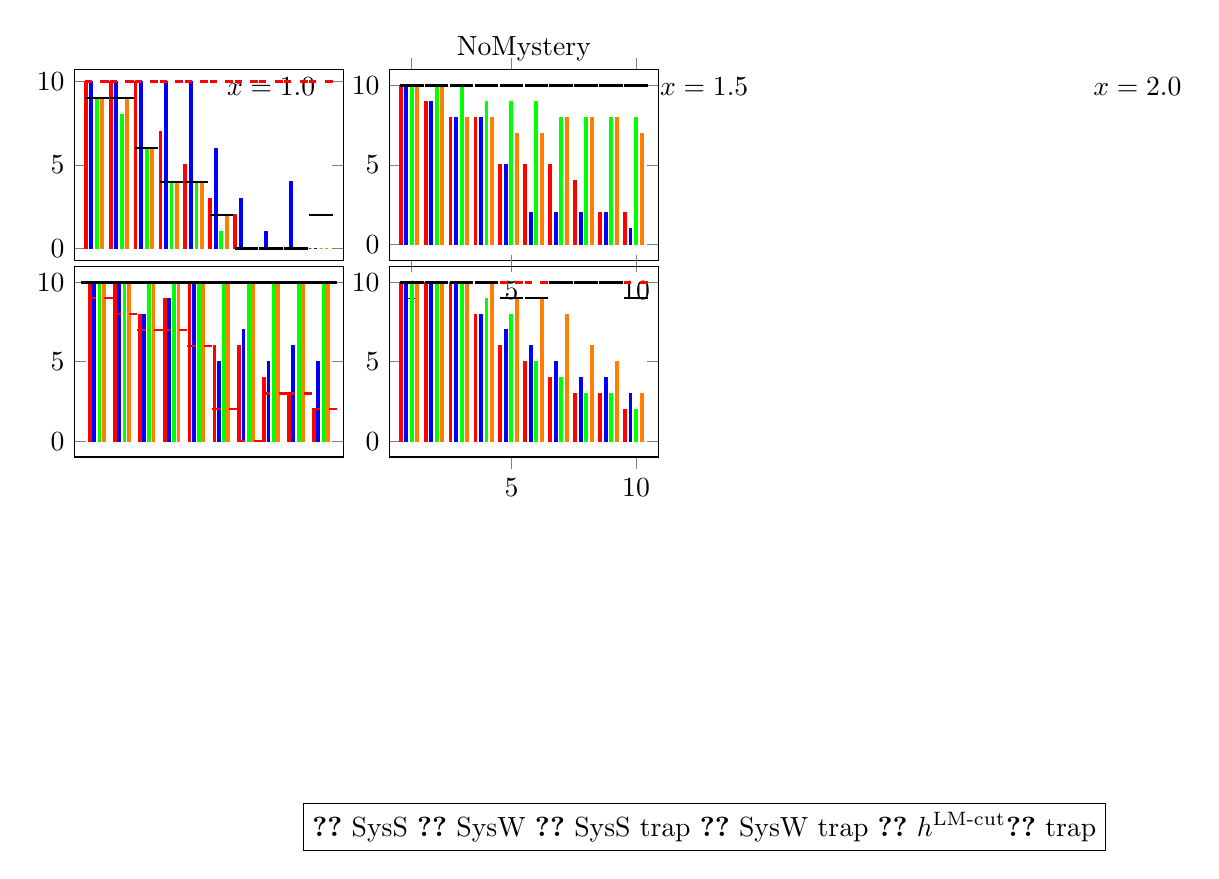
\begin{tikzpicture}
\node[] (c1) at (2.5,2.2) {$x=1.0$};
\node[] (c15) at (8,2.2) {$x=1.5$};
\node[] (c2) at (13.5,2.2) {$x=2.0$};


    \begin{axis}[
    width = 5cm,
    height=4cm,
    enlarge x limits = 0.1,
    enlarge y limits = 0.07,
    legend columns=1,
    ybar,
    bar width=1pt,
    ymin = 0,
    ymax = 10,
	compat=1.6,
	title={},
	xticklabels={,,},
	xtick style={draw=none},
	%ylabel=goals 06,
	at={(0,0)},
]
\addplot+[ybar, bar shift =-4.0pt, red,
]
plot coordinates {
(07, 2) %c_125
(08, 0) %c_125
(03, 10) %c_125
(10, 0) %c_125
(06, 3) %c_125
(09, 0) %c_125
(02, 10) %c_125
(05, 5) %c_125
(04, 7) %c_125
(01, 10) %c_125
};
\label{plot:props_hff_bu_53}
\addplot+[ybar, bar shift =-2.0pt, blue,
]
plot coordinates {
(07, 3) %c_125
(08, 1) %c_125
(03, 10) %c_125
(10, 0) %c_125
(06, 6) %c_125
(09, 4) %c_125
(02, 10) %c_125
(05, 10) %c_125
(04, 10) %c_125
(01, 10) %c_125
};
\label{plot:props_hff_td_53}
\addplot+[ybar, bar shift =0.0pt, green,
]
plot coordinates {
(07, 0) %c_125
(08, 0) %c_125
(03, 6) %c_125
(10, 0) %c_125
(06, 1) %c_125
(09, 0) %c_125
(02, 8) %c_125
(05, 4) %c_125
(04, 4) %c_125
(01, 9) %c_125
};
\label{plot:props_trap_bu_53}
\addplot+[ybar, bar shift =2.0pt, orange,
]
plot coordinates {
(07, 0) %c_125
(08, 0) %c_125
(03, 6) %c_125
(10, 0) %c_125
(06, 2) %c_125
(09, 0) %c_125
(02, 9) %c_125
(05, 4) %c_125
(04, 4) %c_125
(01, 9) %c_125
};
\label{plot:props_trap_td_53}

%lmcut
\addplot+[only marks, mark = -, mark options = {thick, red, dashed}, mark size = 0.15cm, black,
]
plot coordinates {
(02, 10)
(01, 10)
(04, 10)
(03, 10)
(07, 10)
(08, 10)
(06, 10)
(10, 10)
(05, 10)
(09, 10)
};

%trap first meta node top down
\addplot+[only marks, mark = -, mark options = {thick, black}, mark size = 0.15cm, black,
]
plot coordinates {
(01, 9)
(02, 9)
(03, 6)
(04, 4)
(05, 4)
(06, 2)
(07, 0)
(08, 0)
(09, 0)
(10, 2)
};
    \end{axis}
    \hfill
    
%\node[draw, align=center] (test) at (2,-2) {
%\ref{plot:props_hff_bu_53} props-hff-bu\\
%\ref{plot:props_hff_td_53} props-hff-td\\
%\ref{plot:props_trap_bu_53} props-trap-bu\\
%\ref{plot:props_trap_td_53} props-trap-td\\
%};



    \begin{axis}[
    width = 5cm,
    height=4cm,
    enlarge x limits = 0.1,
    enlarge y limits = 0.1,
    legend columns=1,
    ybar,
    bar width=1pt,
    ymin = 0,
    ymax = 10,
	compat=1.6,
	title=NoMystery,
	title style={yshift=-1.5ex},
	%ylabel=goals 6,
	%xticklabels={,,},
	%xtick style={draw=none},
	xtick= {1,5,10},
	at={(4cm,0)},
]
\addplot+[ybar, bar shift =-4.0pt, red,
]
plot coordinates {
(04, 8) %c_100
(09, 2) %c_100
(10, 2) %c_100
(08, 4) %c_100
(02, 9) %c_100
(07, 5) %c_100
(06, 5) %c_100
(05, 5) %c_100
(03, 8) %c_100
(01, 10) %c_100
};
\label{plot:props_bu_hff_46}
\addplot+[ybar, bar shift =-2.0pt, blue,
]
plot coordinates {
(04, 8) %c_100
(09, 2) %c_100
(10, 1) %c_100
(08, 2) %c_100
(02, 9) %c_100
(07, 2) %c_100
(06, 2) %c_100
(05, 5) %c_100
(03, 8) %c_100
(01, 10) %c_100
};
\label{plot:props_td_hff_46}
\addplot+[ybar, bar shift =0.0pt, green,
]
plot coordinates {
(04, 9) %c_100
(09, 8) %c_100
(10, 8) %c_100
(08, 8) %c_100
(02, 10) %c_100
(07, 8) %c_100
(06, 9) %c_100
(05, 9) %c_100
(03, 10) %c_100
(01, 10) %c_100
};
\label{plot:props_bu_trap_46}
\addplot+[ybar, bar shift =2.0pt, orange,
]
plot coordinates {
(04, 8) %c_100
(09, 8) %c_100
(03, 8) %c_100
(08, 8) %c_100
(02, 10) %c_100
(07, 8) %c_100
(06, 7) %c_100
(05, 7) %c_100
(10, 7) %c_100
(01, 10) %c_100
};
\label{plot:props_td_trap_46}

%lmcut
\addplot+[only marks, mark = -, mark options = {thick, red, dashed}, mark size = 0.15cm, black,
]
plot coordinates {
(01, 10)
(02, 10)
(03, 10)
(04, 10)
(05, 10)
(06, 10)
(07, 10)
(08, 10)
(09, 10)
(10, 10)
};

%trap first meta node top down
\addplot+[only marks, mark = -, mark options = {thick, black}, mark size = 0.15cm, black,
]
plot coordinates {
(01, 10)
(02, 10)
(03, 10)
(04, 10)
(05, 10)
(06, 10)
(07, 10)
(08, 10)
(09, 10)
(10, 10)
};
    \end{axis}
    \hfill
    
%\node[draw, align=center] (test) at (8,-18) {
%\ref{plot:props_bu_hff_46} props-bu-hff\\
%\ref{plot:props_td_hff_46} props-td-hff\\
%\ref{plot:props_bu_trap_46} props-bu-trap\\
%\ref{plot:props_td_trap_46} props-td-trap\\
%};



\begin{axis}[
width = 5cm,
height=4cm,
enlarge x limits = 0.1,
enlarge y limits = 0.1,
legend columns=1,
ybar,
bar width=1pt,
ymin = 0,
ymax = 10,
compat=1.6,
at={(0,-2.5cm)},
	xticklabels={,,},
	xtick style={draw=none},
]
\addplot+[ybar, bar shift =-2.5pt, red,
]
plot coordinates {
(08, 4)
(09, 3)
(01, 10)
(03, 8)
(02, 10)
(04, 9)
(05, 10)
(06, 6)
(10, 2)
(07, 6)
};
\label{plot:properties_hff_bu_52}
\addplot+[ybar, bar shift =-1.0pt, blue,
]
plot coordinates {
(01, 10)
(08, 5)
(02, 10)
(04, 9)
(03, 8)
(05, 10)
(06, 5)
(10, 5)
(07, 7)
(09, 6)
};
\label{plot:properties_hff_td_52}
\addplot+[ybar, bar shift =1.0pt, green,
]
plot coordinates {
(09, 10)
(01, 10)
(02, 10)
(04, 10)
(03, 10)
(05, 10)
(06, 10)
(10, 10)
(07, 10)
(08, 10)
};
\label{plot:properties_trap_prefop_bu_52}
\addplot+[ybar, bar shift =2.5pt, orange,
]
plot coordinates {
(01, 10)
(08, 10)
(02, 10)
(03, 10)
(04, 10)
(05, 10)
(06, 10)
(10, 10)
(07, 10)
(09, 10)
};
\label{plot:properties_trap_prefop_td_52}

%start node sysW
\addplot+[only marks, mark = -, mark options = {thick}, mark size = 0.2cm, black,
]
plot coordinates {
(02, 10)
(01, 10)
(04, 10)
(03, 10)
(07, 10)
(08, 10)
(06, 10)
(10, 10)
(05, 10)
(09, 10)
};
%optimal
\addplot+[only marks, mark = -, mark options = {thick, red, dashed}, mark size = 0.2cm, black,
]
plot coordinates {
(03, 7)
(05, 6)
(07, 0)
(09, 3)
(01, 9)
(02, 8)
(04, 7)
(06, 2)
(08, 3)
(10, 2)
};

\end{axis}


    \begin{axis}[
    width = 5cm,
    height=4cm,
    enlarge x limits = 0.1,
    enlarge y limits = 0.1,
    legend columns=1,
    ybar,
    bar width=1pt,
    ymin = 0,
    ymax = 10,
compat=1.6,
%title=c 150,
%ylabel=goals 7,
at={(4cm,-2.5cm)},
]
\addplot+[ybar, bar shift =-4.0pt, red,
]
plot coordinates {
(07, 4) %c_150
(06, 5) %c_150
(05, 6) %c_150
(09, 3) %c_150
(08, 3) %c_150
(10, 2) %c_150
(01, 10) %c_150
(04, 8) %c_150
(03, 10) %c_150
(02, 10) %c_150
};
\label{plot:props_bu_hff_49}
\addplot+[ybar, bar shift =-2.0pt, blue,
]
plot coordinates {
(07, 5) %c_150
(06, 6) %c_150
(05, 7) %c_150
(09, 4) %c_150
(08, 4) %c_150
(10, 3) %c_150
(01, 10) %c_150
(04, 8) %c_150
(03, 10) %c_150
(02, 10) %c_150
};
\label{plot:props_td_hff_49}
\addplot+[ybar, bar shift =0.0pt, green,
]
plot coordinates {
(07, 4) %c_150
(06, 5) %c_150
(05, 8) %c_150
(09, 3) %c_150
(08, 3) %c_150
(03, 10) %c_150
(01, 10) %c_150
(04, 9) %c_150
(10, 2) %c_150
(02, 10) %c_150
};
\label{plot:props_bu_trap_49}
\addplot+[ybar, bar shift =2.0pt, orange,
]
plot coordinates {
(07, 8) %c_150
(06, 9) %c_150
(05, 9) %c_150
(09, 5) %c_150
(08, 6) %c_150
(10, 3) %c_150
(01, 10) %c_150
(04, 10) %c_150
(03, 10) %c_150
(02, 10) %c_150
};
\label{plot:props_td_trap_49}

%lmcut
\addplot+[only marks, mark = -, mark options = {thick, red, dashed}, mark size = 0.15cm, black,
]
plot coordinates {
(02, 10)
(01, 10)
(04, 10)
(03, 10)
(07, 10)
(08, 10)
(06, 10)
(10, 10)
(05, 10)
(09, 10)
};

%trap first meta node top down
\addplot+[only marks, mark = -, mark options = {thick, black}, mark size = 0.15cm, black,
]
plot coordinates {
(01, 10)
(02, 10)
(03, 10)
(04, 10)
(05, 9)
(06, 9)
(07, 10)
(08, 10)
(09, 10)
(10, 9)
};
    \end{axis}
    \hfill
    
%\node[draw, align=center] (test) at (8,-18) {
%\ref{plot:props_bu_hff_49} props-bu-hff\\
%\ref{plot:props_td_hff_49} props-td-hff\\
%\ref{plot:props_bu_trap_49} props-bu-trap\\
%\ref{plot:props_td_trap_49} props-td-trap\\
%};



\node[draw] (test) at (8,-7.2) {
\ref{plot:properties_hff_bu_39}  SysS
\ref{plot:properties_hff_td_39}  SysW
\ref{plot:properties_trap_prefop_bu_39} SysS trap 
\ref{plot:properties_trap_prefop_td_39} SysW trap 
\ref{plot:baseline_lmcut} \hlmcut
\ref{plot:baseline_sysW_node} trap
};
\end{tikzpicture}

\end{document}
